\section{Splay-дерево: определение и практическая значимость.}

\textbf{Опр} Сплей-дерево (англ. Splay-tree) — это двоичное дерево поиска. Оно позволяет находить быстрее те данные, которые использовались недавно.

\textbf{Практическая значимость } Splay-дерево замечательно тем, что если к какому-то элементу делалось большое количество запросов, то этот элемент будет находиться ближе к корню дерева, т.е. на запросы к этому элементу мы сможем отвечать быстрее.

Допустим, у нас имеется какая-то база данный, в который мы хотим задавать вопросы. Например, мы пишем какой-то сайт, и нам нужно хранить список элементов вида 'пользователь-хэш пароля' , чтобы проверять, правильный ли пароль вводит пользователь. Мы храним большой объем информации. И хранить это естественно в виде дерева поиска.

На сайте есть пользователи, который заходят часто, а есть те, которые заходят редко. Тогда логично, что пользователей, которые заходят часто, нужно хранить ближе к корню, чтобы быстрее отвечать на запросы. 

Для этого используют splay-деревья. Когда происходит запрос к элементу, он поднимается в корень, и если к этому же элементу поступил повторный запрос, то этот элемент не успел спуститься вглубь дерева, и для выполнения запроса нам нужно спуститься не так глубоко.

\section{Splay-дерево: операции zig, zig-zig и zig-zag, операция splay.}

\textbf{Splay } - операция, которая выполняет подъем элемента дерева в корень. Сама она разбивается на 3 подзадачи:

\begin{itemize}
    \item [1] \textbf{zig}
    
    Если p — корень дерева с сыном x, то совершаем один поворот вокруг ребра (x,p), делая x корнем дерева. Данный случай является крайним и выполняется только один раз в конце, если изначальная глубина x была нечетной. 
    
    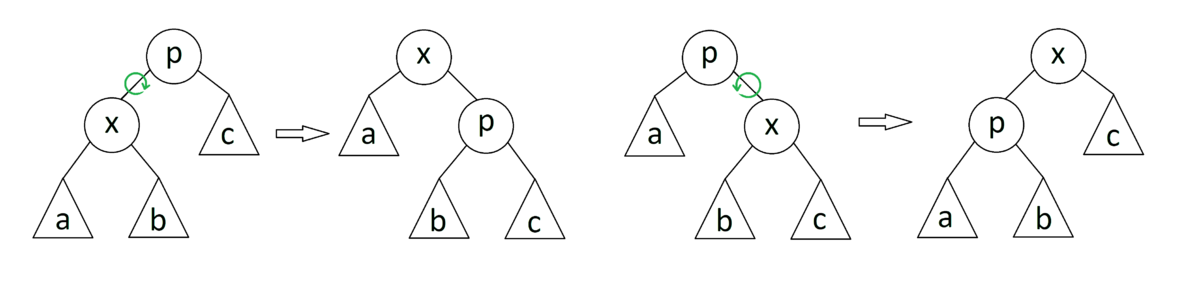
\includegraphics[width = 10cm]{images/47-50_зиг}
    
    \textbf{Замечание } Это то же самое, что левый (правый) маленький поворот
    
    \item[2] \textbf{zig-zig}
    
    Если p — не корень дерева, а x и p — оба левые или оба правые дети, то делаем поворот ребра (p,g), где g отец p, а затем поворот ребра (x,p).
    
    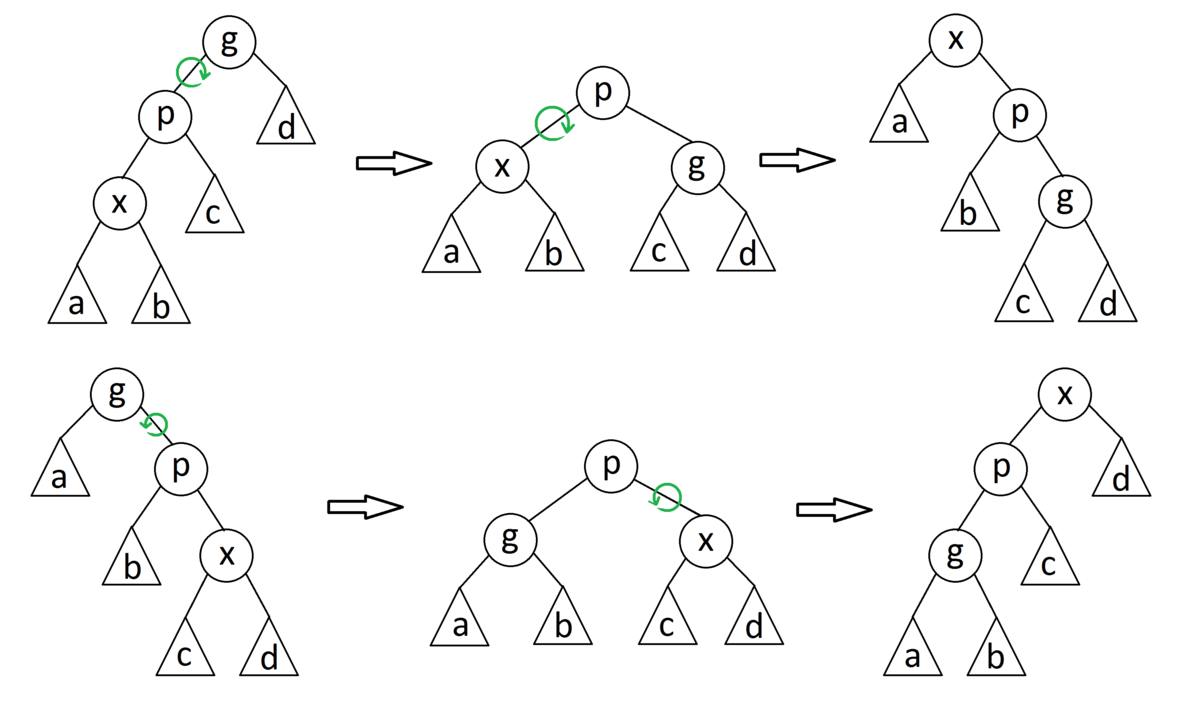
\includegraphics[width = 10cm]{images/47-50_pиг_зиг}
    
    \item[3] \textbf{zig-zag}
    
    Если p — не корень дерева и x — левый ребенок, а p — правый, или наоборот, то делаем поворот вокруг ребра (x,p), а затем поворот нового ребра (x,g), где g — бывший родитель p.
    
    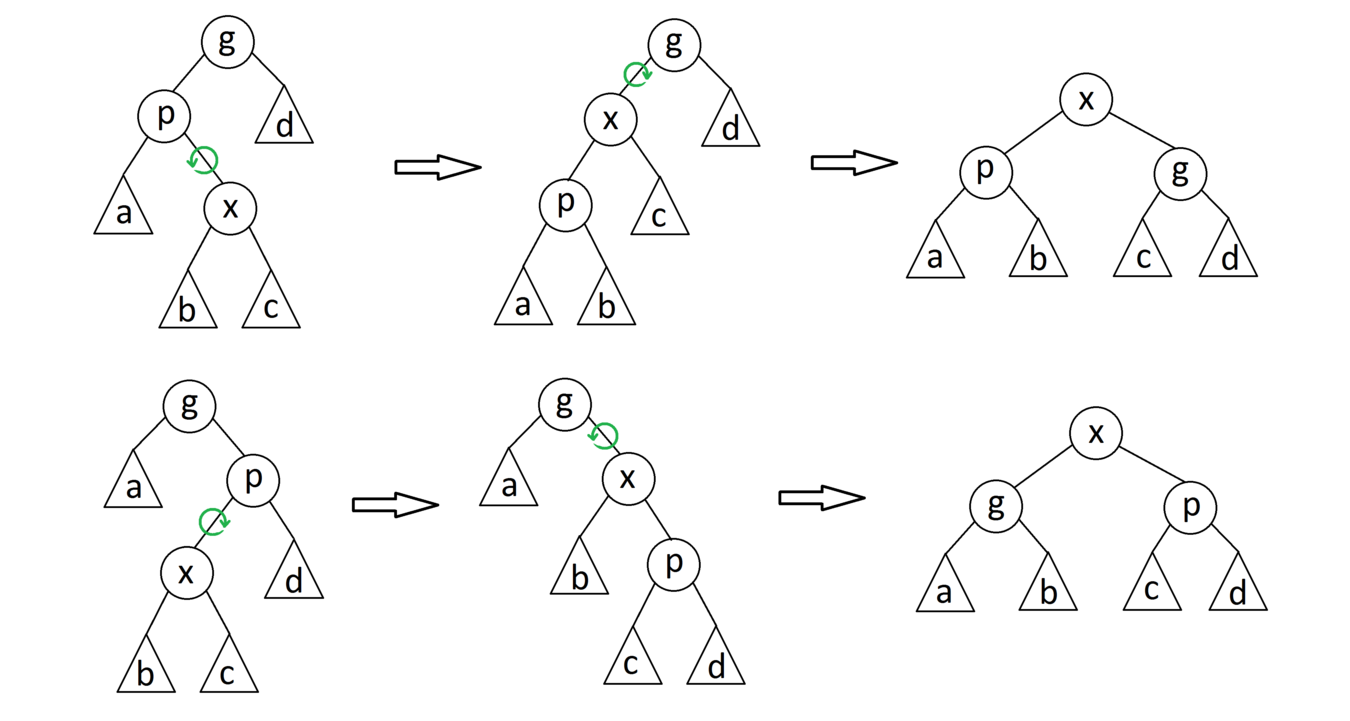
\includegraphics[width = 10cm]{images/47-50_зиг_заг2}
    
     \textbf{Замечание } Это то же самое, что левый (правый) большой поворот
\end{itemize}

Таким образом, чтобы поднять элемент X  в корень дерева, нужно произвести какую-то комбинацию zig-zig и zig-zag, а в конце, возможно, сделать один zig.
\section{Амортизированное время работы операции splay с помощью метода потенциалов.}

\subsection*{Метод потенциалов}

Для некоторого состояния структуры S вводим потенциал $\Phi(S)$— это функция от состояния структуры.

Изначально потенциал равен $\Phi_0$, а после выполнения i-й операции - $\Phi_i$.
$t_i$ - реальное время работы i-й операции, тогда амортизированное время работы операции:  $a_i$ = $t_i$ + $\Phi_i - \Phi_{i-1} $.

Тогда $a_1 + a_2 + ... + a_q  = t_1 + t_2 + ... + t_q + (\Phi_1 - \Phi_0) + (\Phi_2 - \Phi_1) + ... + (\Phi_q - \Phi_{q-1}) = \displaystyle\sum_{i=1}^{q} t_i + \Phi_q - \Phi_0$

Если $\Phi_q - \Phi_0$ >= 0, то получаем то, что нам нужно:

$\displaystyle\sum_{i=1}^{q} t_i$ <= $\displaystyle\sum_{i=1}^{q} a_i$ 

Т.е. реальное время работы не превосходит амортизированного.

\subsection*{Оценка времени работы операции splay}
\textbf{Теорема} Амортизированное время работы операции  splay есть О(log(n)).

$\blacktriangle$
Положим S(x) - количество элементов в поддереве x (x  включается в поддерево),

r(x) = $\log_{2}{S(x)}$

$\Phi(x) = \displaystyle\sum_{x - vertex} r(x)$

Давайте рассмотрим i-ую операцию, на которой происходит splay(x)
Покажем, что $a_i <= 1 + 3( r'(x) - r(x)) <= 1 + 3*\log_{2}{n}$, где r'(x) - ранг x  в новом дереве, r(x) -ранг x  в старом дереве.

После операции splay x переходит в корень, поэтому r'(x) = $\log_{2}{n}$ $\Longrightarrow$ $a_i <= O(\log_{2}{n})$

Теперь рассмотрим амортизированное время работы операций zig, zig-zig, zig-zag:
\begin{itemize}
    \item \textbf{zig}
    
    $a(zig) = 1 + r'(x) + r'(p) - r(x) - r(p)$

$r'(p) <= r(p)    \Longrightarrow     a(zig) <= 1 + r'(x) - r(x) <= 1 + 3(r'(x) - r(x))$

\item \textbf{zig-zig}

$a(zig-zig) = 2 + r'(x) + r'(p)  + r'(g)- r(x) - r(p) - r(g)$

$r'(x) = r(g), r(p) >= r(x), r'(p) <= r'(x)  \Longrightarrow $

$a(zig-zig) <= 2 + r'(x)  + r'(g)- 2*r(x) $

Проверим, выполняется ли, что 

$ 2 + r'(x)  + r'(g)- 2*r(x) <= 3(r'(x) - r(x))$

$ r'(g) + r(x) - 2*r'(x) <= -2$


$ \log_{2}{\frac{S'(g)}{S'(x)}} + \log_{2}{\frac{S(x)}{S'(x)}} <= -2$

$\frac{S'(g)}{S'(x)} = a, \frac{S(x)}{S'(x)} = b $

Покажем, что a + b <=1

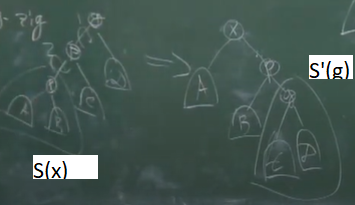
\includegraphics[width = 7cm]{images/47-50_zzp}

Понятно, что каждый блок содержит меньше элементов, чем S'(x), при этом они не пересеекаются, поэтому a + b <= 1. Из неравенства о среднем геометрическом ab <= 1/4 $ \Longrightarrow $ неравенство верно.

\item \textbf{zig-zag}

$a(zig-zag) = 2 + r'(x) + r'(p)  + r'(g)- r(x) - r(p) - r(g)$

$r'(x) = r(g), r(p) >= r(x) \Longrightarrow $

$a(zig-zag) <= 2 + r'(p) + r'(g) - 2*r(x)$

Проверим, выполняется ли, что 

$ 2 + r'(p) + r'(g) - 2*r(x) <= 2(r'(x) - r(x))$    $\Leftrightarrow$

$r'(p) + r'(g) - 2*r'(x) <= -2$
$\Leftrightarrow$

$ \log_{2}{\frac{S'(g)}{S'(x)}} + \log_{2}{\frac{S'(p)}{S'(x)}} <= -2$

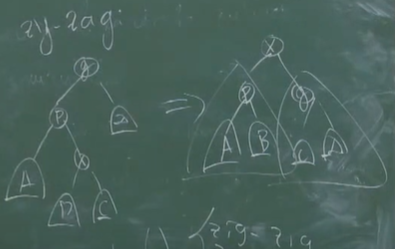
\includegraphics[width = 7cm]{images/47-50_zzp@}

Тут доказывается аналогично прерыдущему пункту. Таким образом

$ 2 + r'(p) + r'(g) - 2*r(x) <= 2(r'(x) - r(x)) <= 3((r'(x) - r(x)))$

\end{itemize}

Отсюда следует, что каждая операция выполняется не более чем за $1 + 3( r'(x) - r(x))$. Сложим все операций, которые выполняли для того чтобы поднять элемент x:

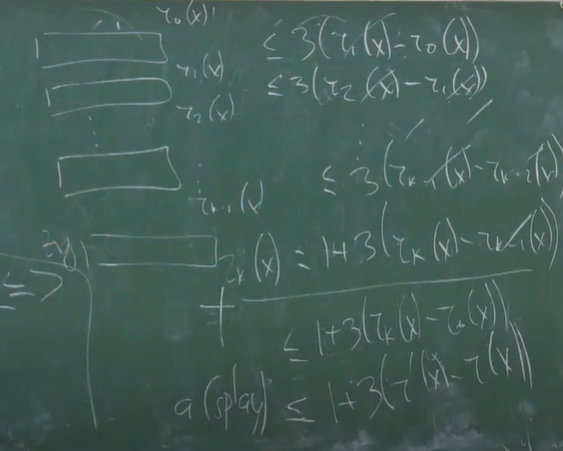
\includegraphics[width = 7cm]{images/47-50_zzzend}

В результате получим то, что нужно.
$\blacksquare$

\section{Splay-дерево: реализация insert, erase и find, связь с операцией splay, оценка времени работы.}

\subsection*{Insert }

Находим, куда нам нужно вставить x в дереве, запускаем splay от этого элемента, как это делали в обычном дереве, а потом вызываем splay от x. 

\textit{Асимптотика: Время insert ограниченно сверху временем работы splay. Амортизированное время работы: O(log(n))}

Другая реализация - через split. Запускаем split(tree, x), который нам возвращает деревья tree1 и tree2, их подвешиваем к x как левое и правое поддеревья соответственно.


\subsection*{Erase }

Поступаем точно так же, как делали в обычном бинарном дереве: разбиваем ситуацию на 3 случая, в зависимости от количества детей, но после того, как удаление произошло, запускаем splay от самой глубокой посещенной вершины.

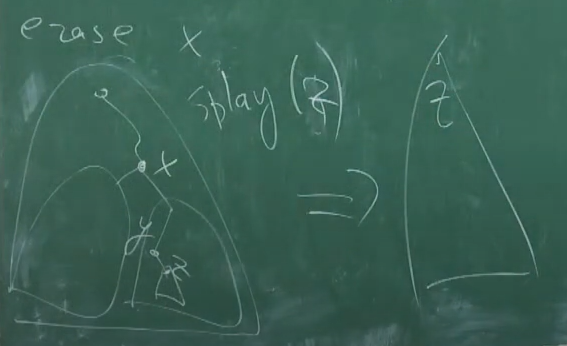
\includegraphics[width = 7cm]{images/47-50_erase}

Здесь y - наименьший элемент в поддреве, и у него есть правый сын

\textit{Асимптотика: Время erase ограниченно сверху временем работы splay. Именно поэтому мы делаем splay от самой глубокой посещенной вершины. Амортизированное время работы: $O(\log(n))$}

\subsection*{Find }

Эта операция выполняется как для обычного бинарного дерева поиска, только после нее запускается операция splay от найденного элемента.

\textit{Асимптотика: как и в прерыдущих случаях, время работы оценивается сверху временем работы splay, поэтому: амортизированное O(log(n))}